\chapter{Implementatie}

\section{Technologi\"en}

Wij hebben gekozen voor de volgende technologi\"en voor het ontwikkelen van deze webapplicatie:
\begin{itemize}
	\item Groovy - Een dynamische en behendig object geori\"enterd taal gebaseerd op de taal Java.
	\vspace{2mm} \\
	\textit{Wij hebben hiervoor gekozen omdat Java niet de meest prettig taal is om mee te ontwikkelen maar de Java Virtual Machine, waar Groovy ook op draait, heel stabiel en veilig is. Groovy is maakt gebruikt van de sterkt punten van Java en verbetert de tekorkommingen.}

	\item Grails - Een webframework voor Groovy met de motto ``Convention over configuration''. Het is gefocused op het snel en makkelijk opzetten van webapplicaties.
	\vspace{2mm} \\
	\textit{Wij hebben hiervoor gekozen omdat dit het best ontwikkeld en langst bestand webframework is voor Groovy. Hun ontwikkelings filosofie maakte het ons ook makkelijk om een werkend webapplicatie te maken binnen beperkt tijd.}

	\item Vaadin - Een framework om moderne graphical user interfaces voor webapplicaties te bouwen.
	\vspace{2mm} \\
	\textit{Wij hebben hiervoor gekozen omdat Vaadin het makkelijk maakt om interfaces te maken en tegelijke tijd alle controle over te houden.}
\end{itemize}

\section{Componenten}

\subsection{Checkin}

\begin{figure}[here]
	\centering
	\includegraphics{Images/incheck.png}
	\caption{Checkin voor studenten}
	\label{fig:checkin-student}
\end{figure}

\begin{figure}[here]
	\centering
	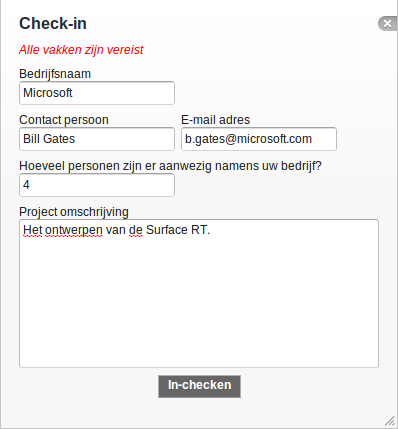
\includegraphics[width=0.8\textwidth]{Images/checkin-company.png}
	\caption{Checkin voor bedrijven}
	\label{fig:checkin-bedrijf}
\end{figure}
